\documentclass[10pt,a4paper]{scrartcl}
\usepackage[utf8]{inputenc}
\usepackage[T1]{fontenc}
\usepackage[ngerman]{babel}
\usepackage{microtype, multicol, marginnote, bera, parskip}
\usepackage{listings, amsmath, amssymb, graphicx, tikz, epic}
\usepackage{stmaryrd} %for lightning arrow
\usepackage{pstricks, pst-node, pst-tree, pdflscape}
\usepackage[babel=true]{csquotes}
\usepackage{placeins}
\tolerance=2000
\setcounter{secnumdepth}{0}
\usepackage[inner=2.5cm,outer=2.5cm,top=1.5cm,bottom=1.5cm,includeheadfoot]{geometry}
\newcommand{\subExercise}[1]{\vspace{1em} \noindent{\bf #1)}}
\author{Michael Mardaus \and Andrey Tyukin}
\title{
\includegraphics[scale=0.2]{../logo_schriftzug}\\
Technische Informatik: Abgabe 3}

\begin{document}

\maketitle

\section*{Exercise 3.1 (MUX Wizardry)}

\subExercise{a}  
We can construct a $n$-MUX from a $1$-MUX and 
two $(n-1)$-MUX'es, clamping the two larger MUX'es to the inputs of the $1$-MUX. 
A trivial induction immediately yields that we need $2^n - 1$ $1$-MUX'es 
to construct a $n$-MUX in that way. For example, for a $4$-MUX we need $15$ 
$1$-MUX'es:

\vspace{1em}
\begin{figure}[h]
  \centering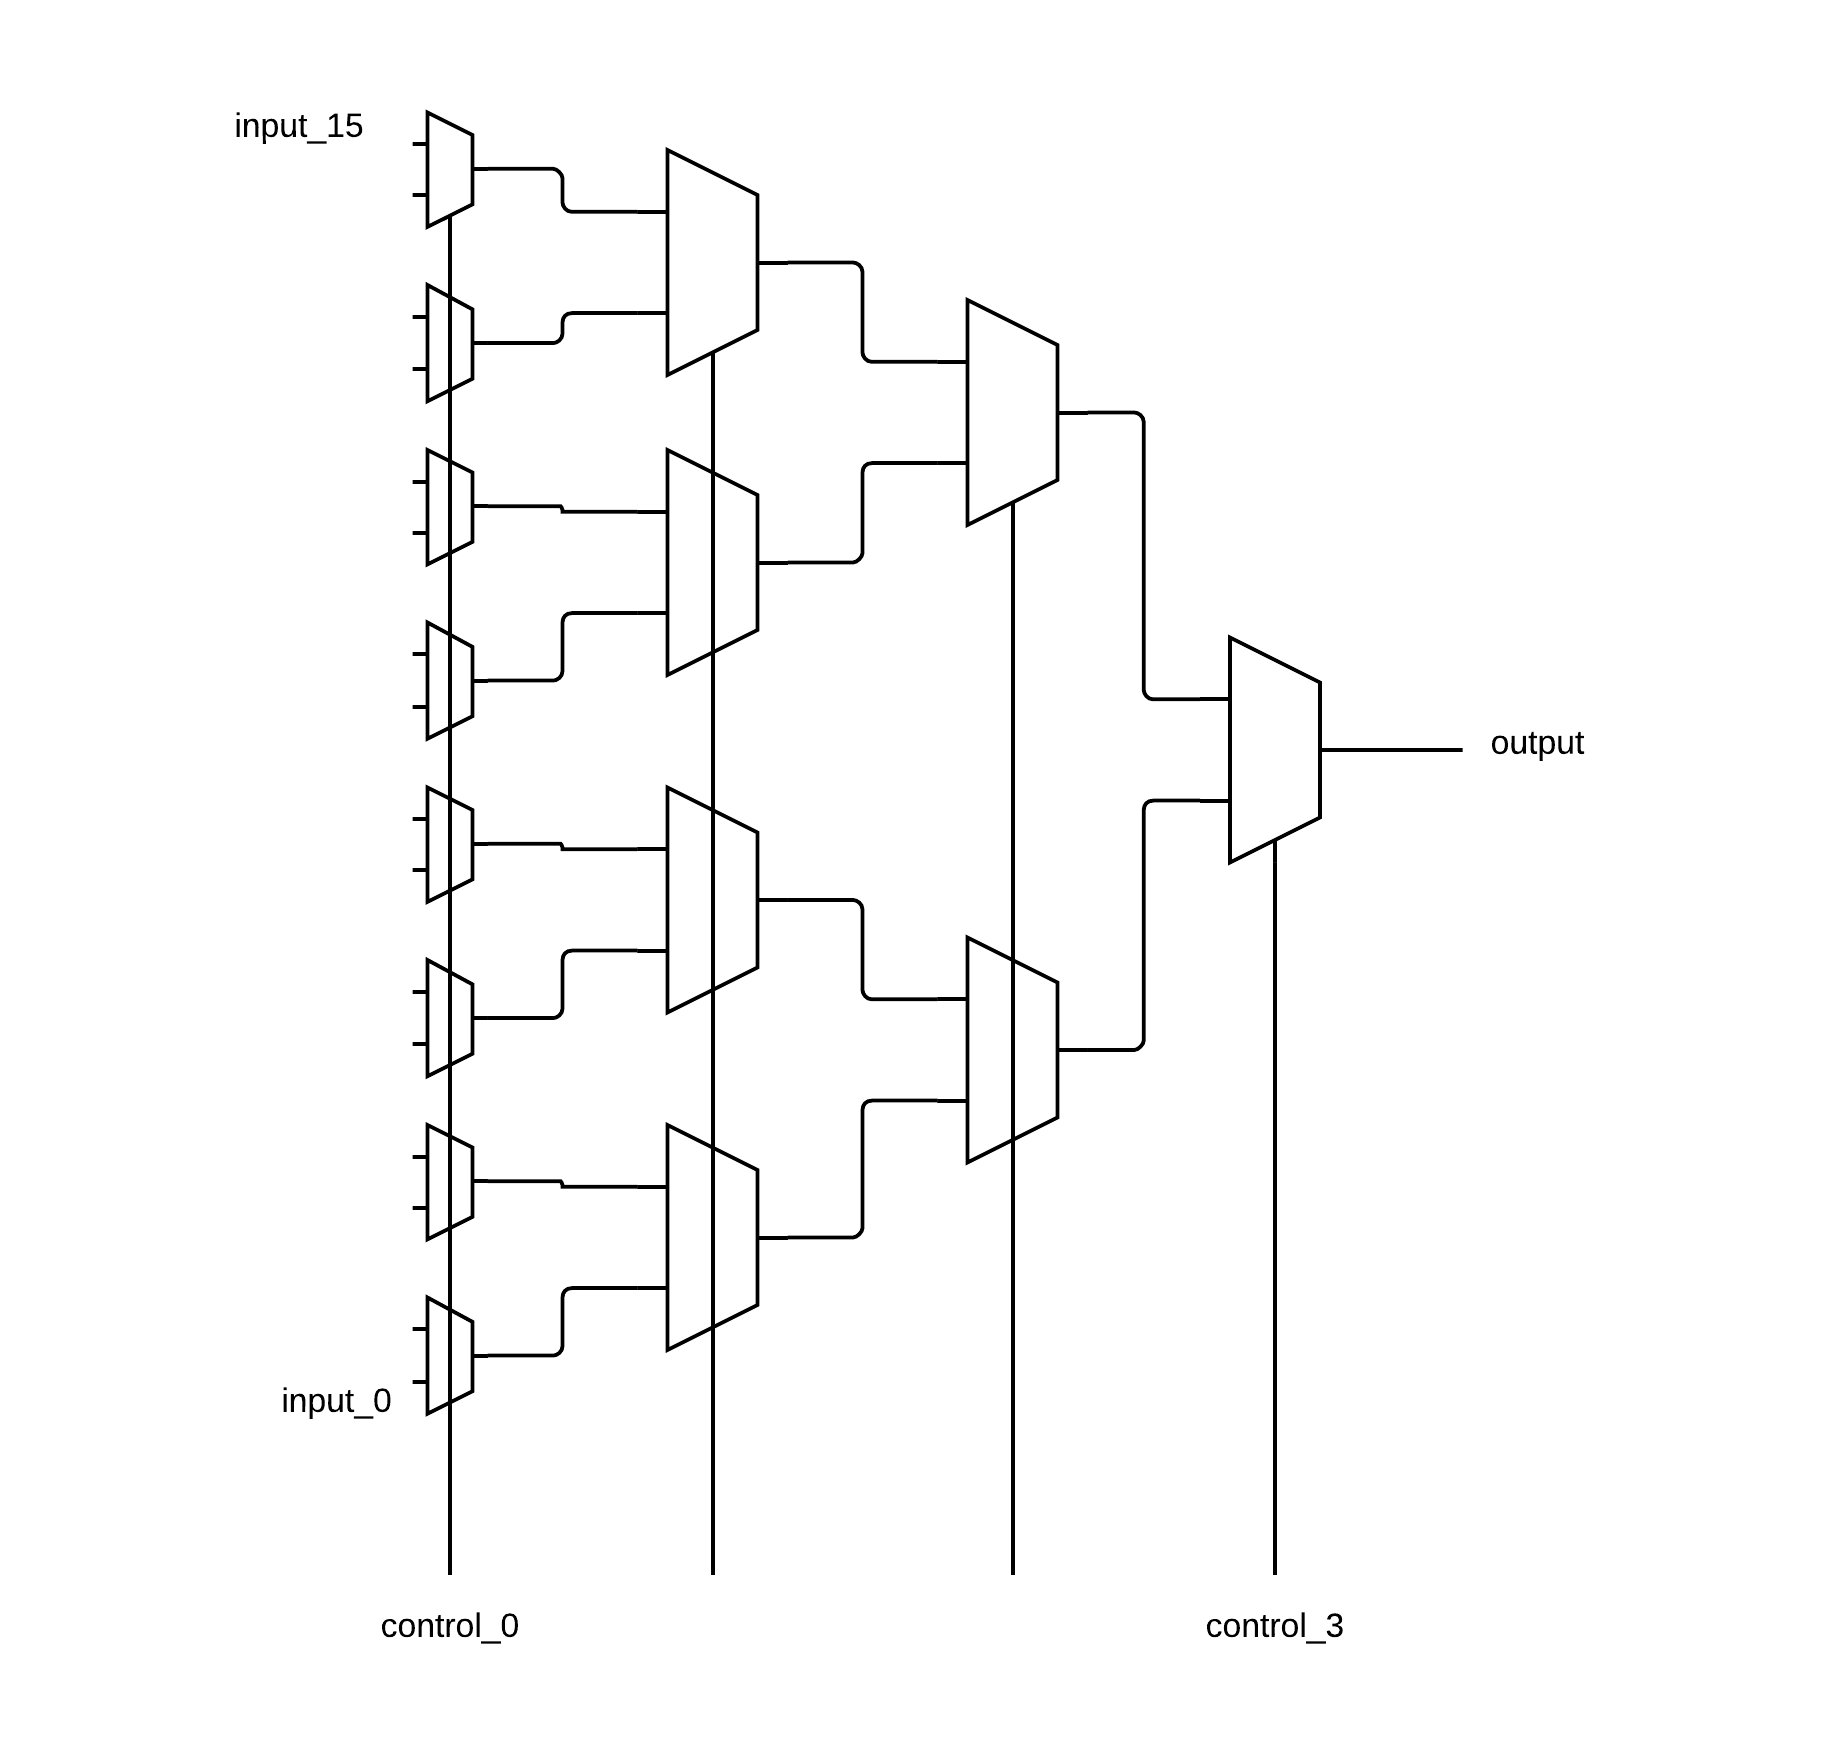
\includegraphics[width=0.6\linewidth]{images/mux4FromMux1.png}
  \caption{Solution to 1 (a)}
\end{figure}
\vspace{1em}

\subExercise{b}
We have $f = m_0 + m_3 + m_6 + m_{13}$. 
(Notice that we read the numbers from right to left, interpreting $x_4$ as least 
significant bit and $x_1$ as most significant bit).

All we have to do is to mark the corresponding inputs with ones (notice that
the order of control signals $x_1$ to $x_4$ corresponds to reading the numbers 
from right to left, the topmost input corresponds to the least significant bit).
\vspace{1em}
\begin{figure}[h]
  \centering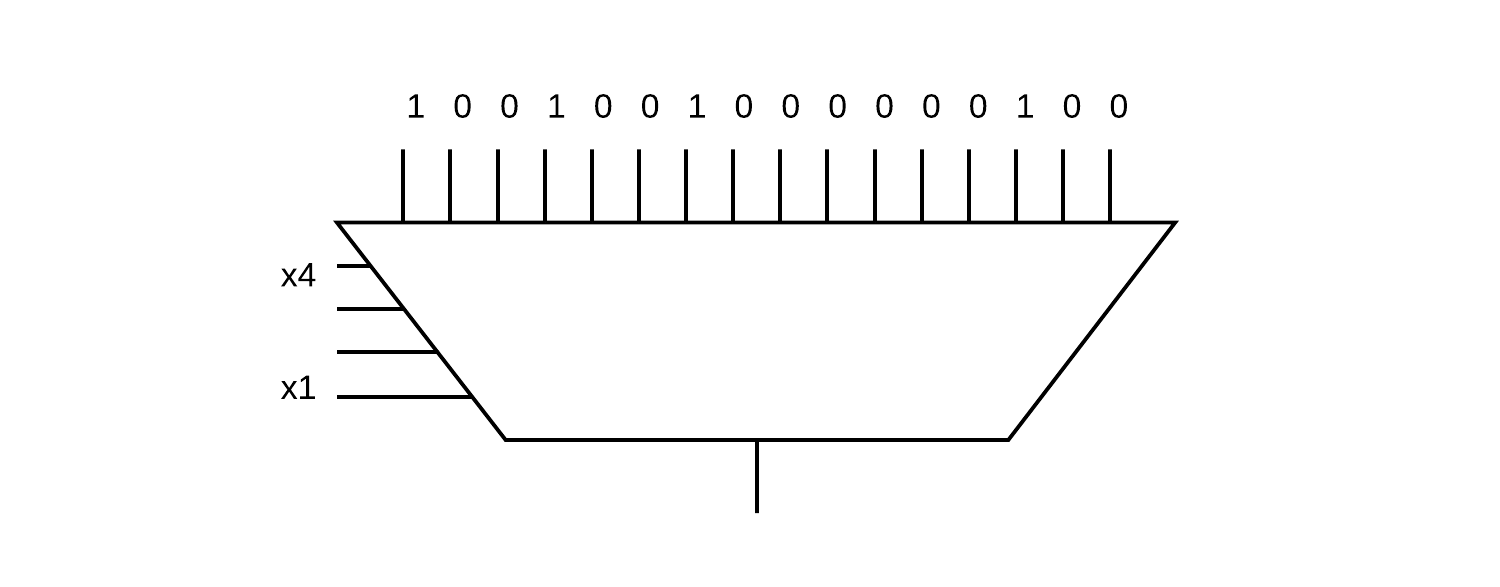
\includegraphics[width=0.7\linewidth]{images/tiExercise3-1-b.png}
  \caption{Solution to 1 (b)}
\end{figure}
\vspace{1em}

\subExercise{c}
Our goal is to implement the function from part b) with only two 2-MUX'es and one inverter.
To derive the optimized circuit, we need some notation. We shall denote an N-MUX as follows:
\[
  MUX_{c_0, \dots, c_{N-1}}\left(i_0, \dots, i_{2^N-1}\right) := 
  \bigvee\limits_{k = 0}^{2^N-1}i_k m_k\left(c_0, \dots, c_{2^N-1}\right).
\]
where $m_k$ is the $0$-indexed minterm.
More concretely, for 2-MUX we use the notation:
\[
  MUX_{l,h}(a,b,c,d) := a\bar h \bar l + b \bar h l + c h \bar l + d h l.
\]
Notice that from this definition and idempotence it immediately follows:
\[
  MUX_{l,h}(a,b,c,d) = MUX_{l,h}(a,b\bar h, c, d h). \qquad (\ast)
\]
Using this, we calculate:
\begin{align*}
f(x_1,x_2,x_3,x_4) =&
  \bar x_1 \bar x_2 \bar x_3 \bar x_4 + 
  \bar x_1 \bar x_2 x_3 x_4 + 
  \bar x_1 x_2 x_3 \bar x_4 + 
  x_1 x_2 \bar x_3 x_4  \\
  \overset{\textrm{def MUX}}{=}&
  MUX_{x_2,x_1}\left(\bar x_3 \bar x_4 + x_3 x_4, x_3 \bar x_4, 0, \bar x_3 x_4 \right) \\
  \overset{\textrm{def XOR}}{=}&
  MUX_{x_2,x_1}\left(
    \neg(x_3 \not \leftrightarrow x_4),
    (x_3 \not \leftrightarrow x_4) x_3, 
    0, 
    (x_3 \not \leftrightarrow x_4) x_4
  \right) \\
  \overset{(\ast) \textrm{, idempotence}}{=}&
  MUX_{x_2,x_1}\left(
    \neg(x_3 \not \leftrightarrow x_4),
    (x_3 \not \leftrightarrow x_4) x_3 \bar x_1 \bar x_1, 
    0, 
    (x_3 \not \leftrightarrow x_4) x_4 x_1 x_1
  \right) \\
  \overset{+0}{=}&
  MUX_{x_2,x_1}\left(
    \neg(x_3 \not \leftrightarrow x_4),
    MUX_{x_1, (x_3 \not \leftrightarrow x_4)}\left(0,0,x3,x4\right)\bar x_1, 
    0, 
    MUX_{x_1, (x_3 \not \leftrightarrow x_4)}\left(0,0,x3,x4\right)x_1
  \right) \\
  \overset{(\ast)}{=}&
  MUX_{x_2,x_1}\left(
    \neg(x_3 \not \leftrightarrow x_4),
    MUX_{x_1, (x_3 \not \leftrightarrow x_4)}\left(0,0,x3,x4\right), 
    0, 
    MUX_{x_1, (x_3 \not \leftrightarrow x_4)}\left(0,0,x3,x4\right)
  \right)
\end{align*}
In the step marked as "+0" we used two transformations of the type
\[
(x_3 \not \leftrightarrow x_4) x_3 \bar x_1 = 
(0 + 0 + x_3(x_3 \not \leftrightarrow x_4)\bar x_1 + 
         x_4(x_3 \not \leftrightarrow x_4)x_1)\bar x_1 = 
MUX_{x_1, (x_3 \not \leftrightarrow x_4)}\left(0,0,x3,x4\right)\bar x_1
\]
two times.
Now we can replace the $XOR$ expression by another MUX, and obtain the
following circuit:
\vspace{1em}
\begin{figure}[h]
  \centering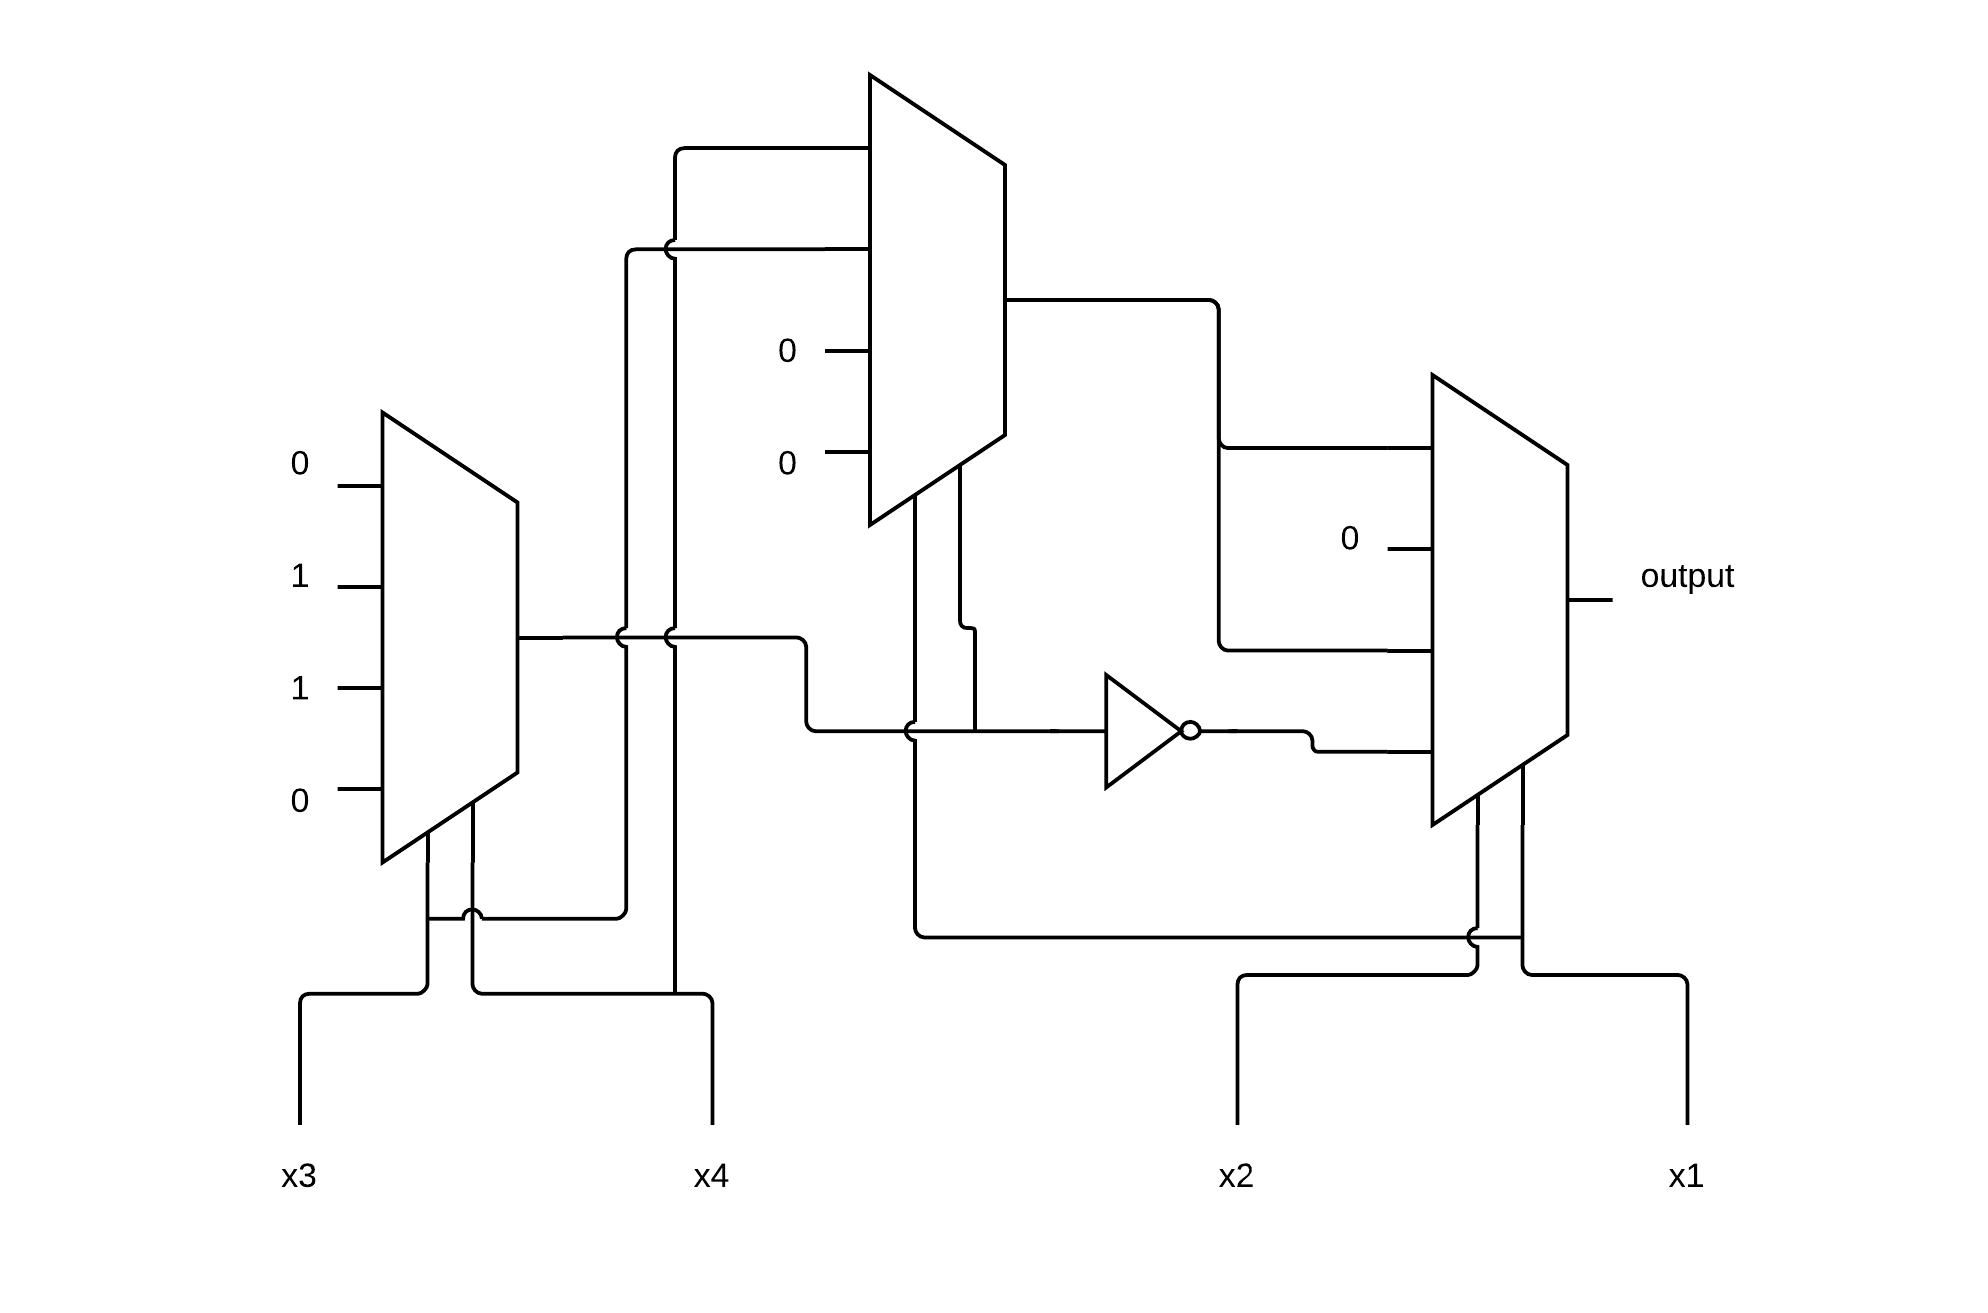
\includegraphics[width=\linewidth]{images/exercise_3_1_c.png}
  \caption{Solution to 3.1 (c)}
\end{figure}
\vspace{1em}

\FloatBarrier
% Exercise 2.2
\section*{Exercise 2 (Air conditioner)}
E-mail sent to tutors, awaiting clarification of the question.

\section*{Exercise 3: MUX is universal}

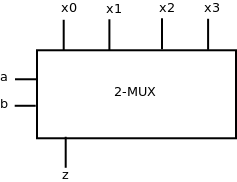
\includegraphics[width=3cm]{images/3-3.png}
\begin{enumerate}
 \item AND: $x_0=x_1=x_2=0$ and $x_3 = 1$ yields output $z = a \land b$
 \item OR: $x_0 = 0$ and $x_1=x_2=x_3= 1$ yields output $z = a \lor b$
 \item NOT: since NOT is an unary operand $b=0$ and $x_0=1, x_1=0, (x_2=x_3=0)$ yields output $z = \lnot a$
\end{enumerate}

\section*{Exercise 4 (4-DeMUX from smaller parts)}
If we want to construct a 4-DeMUX, but have only 4 2-DeMUX'es and infinite number of
simpler gatters at our disposal, we can construct an additional 2-DeMUX from scratch
from simpler AND gatters and inverters, and then clamp the four 2-DeMUX'es to it's 
outputs:
\vspace{1em}
\begin{figure}[h]
  \centering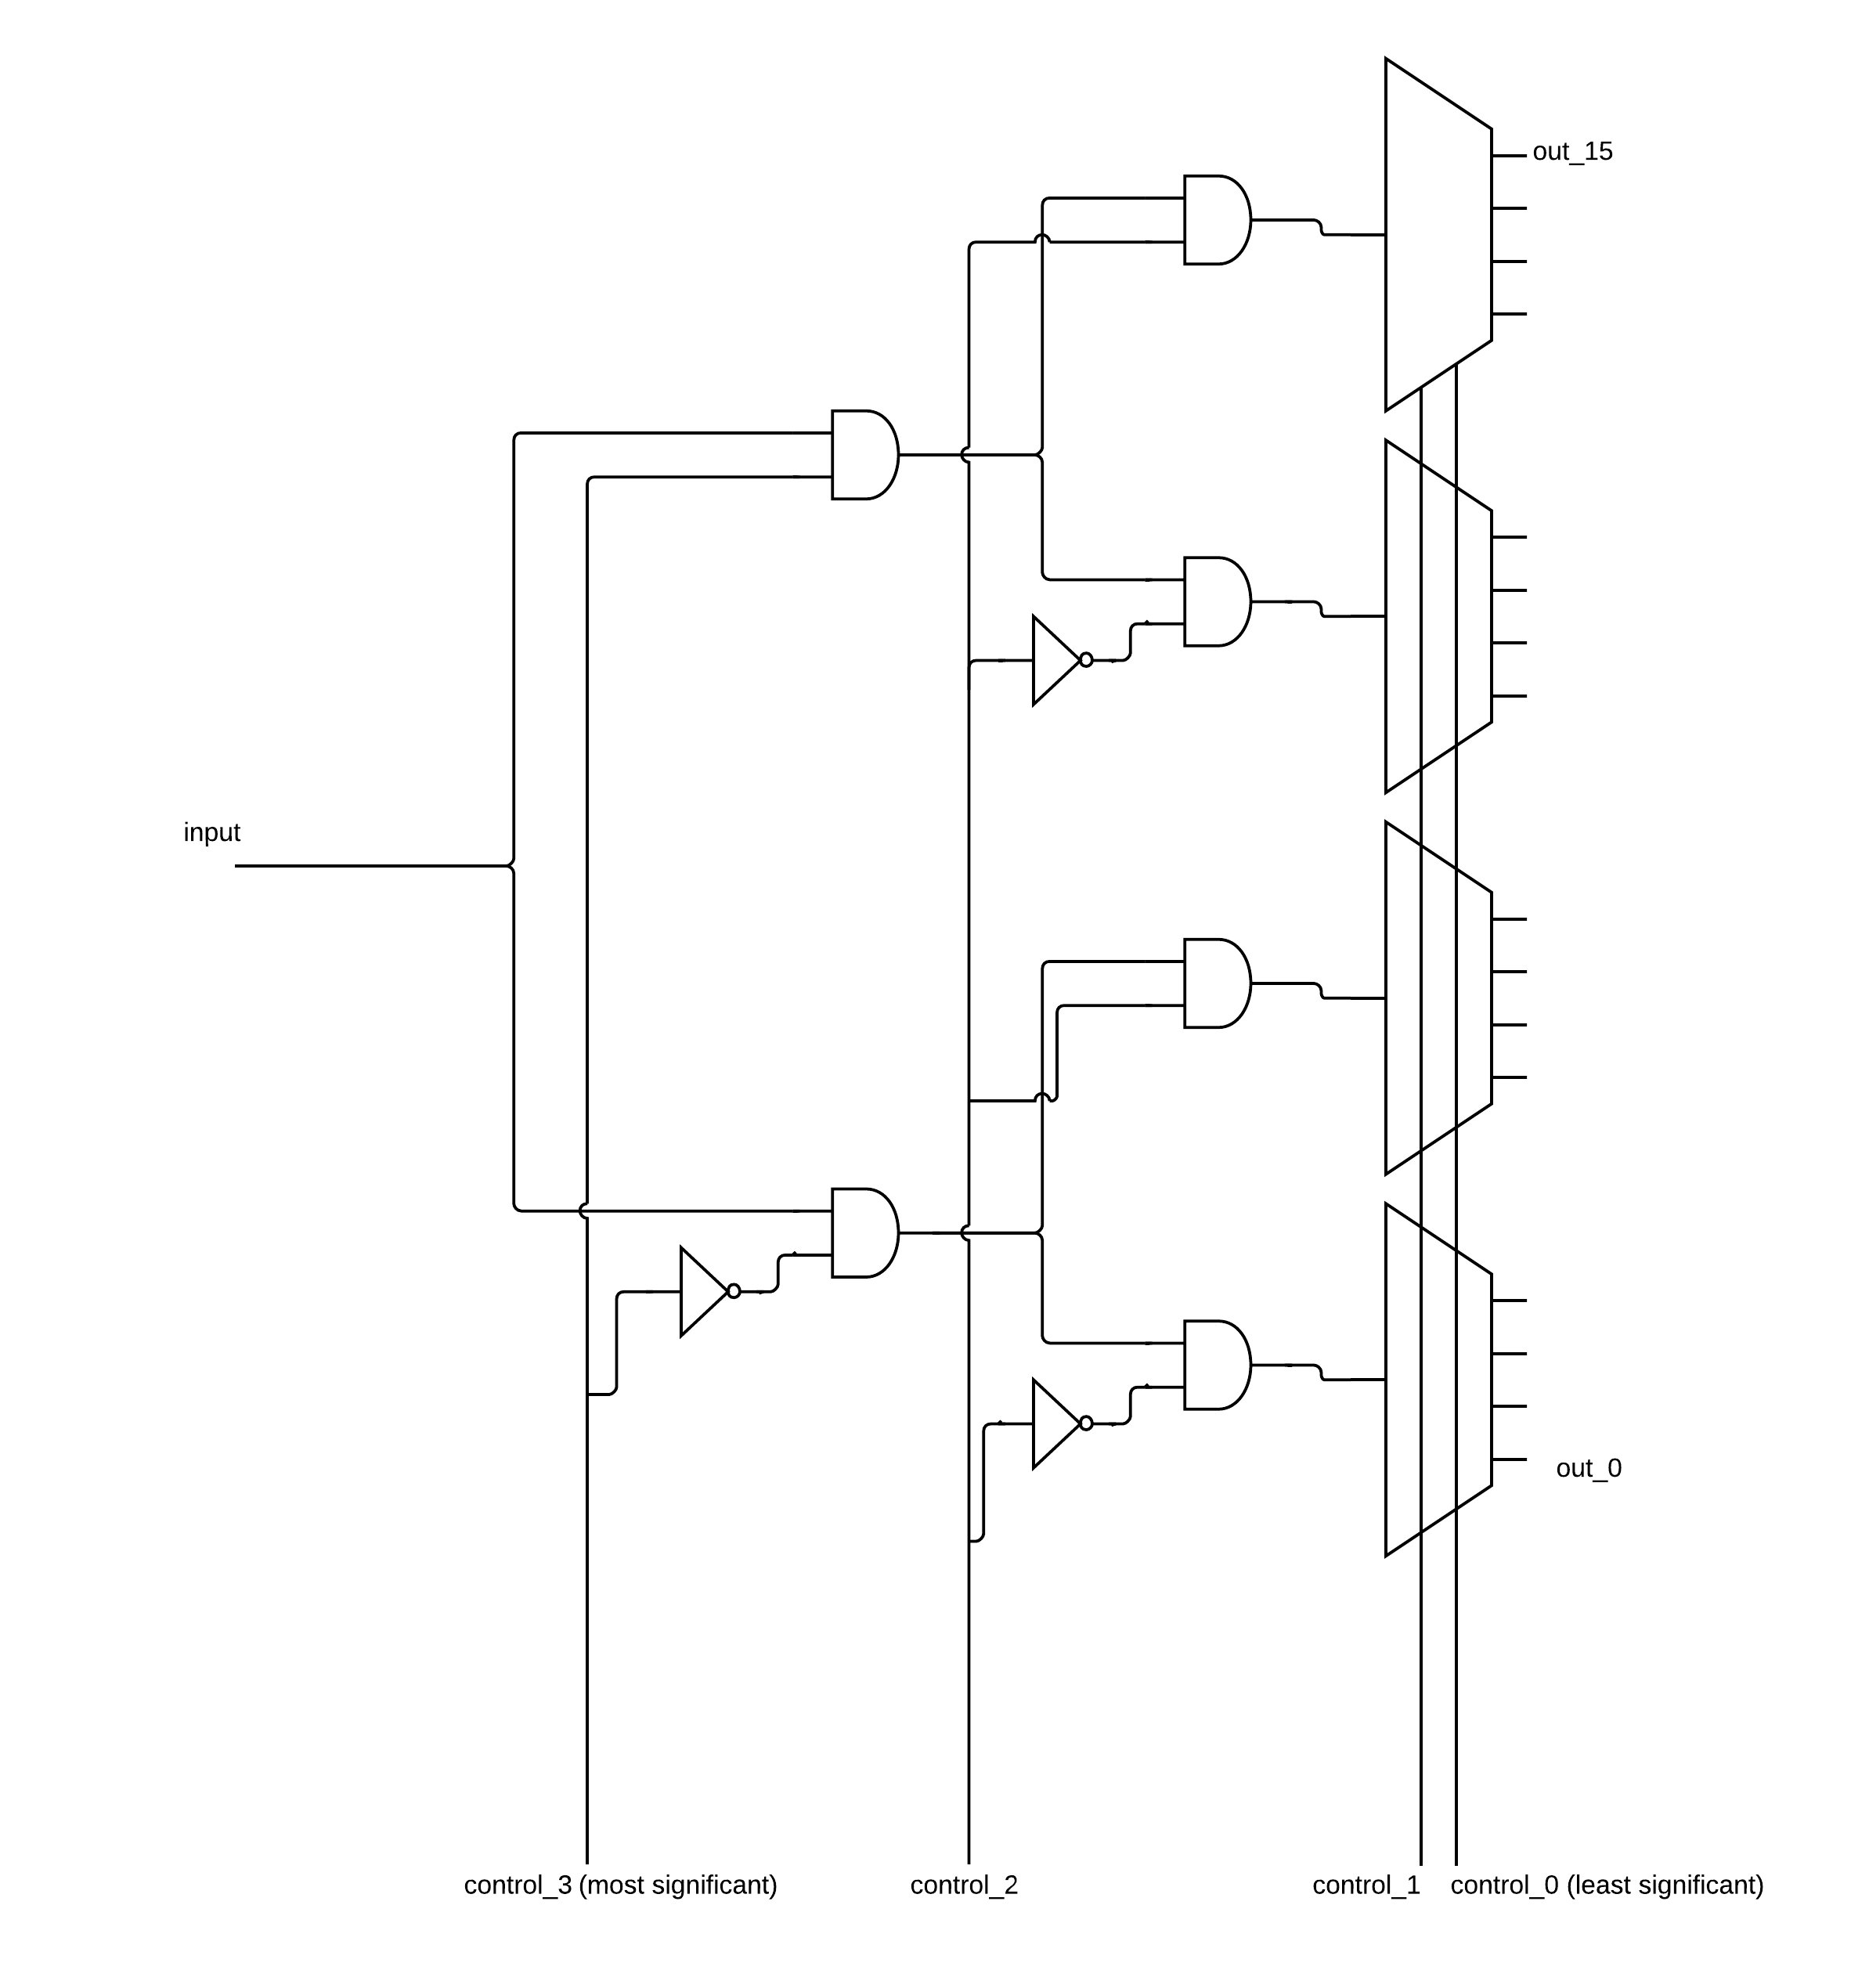
\includegraphics[width=\linewidth]{images/exercise_3_4.png}
  \caption{Solution to 3.4}
\end{figure}
\vspace{1em}

\end{document}
